\documentclass[]{ctexart}
\usepackage[]{graphicx}
\graphicspath{{pictures}}
\title{基本MOS器件物理 Basic MOS Device Physics}
\begin{document}

\section{MOSFET}
\subsection{MOSFET结构}
    \begin{figure}[ht]
        \centering
        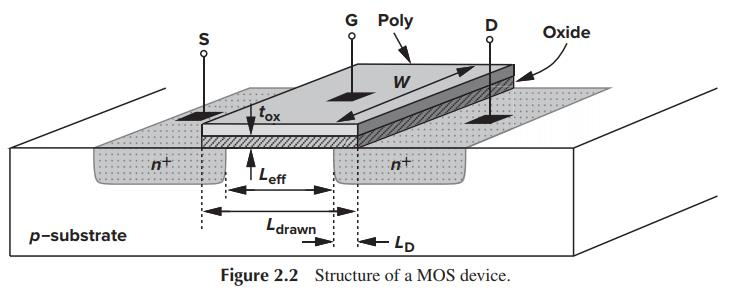
\includegraphics[scale=0.6]{MOSFET_Strcture}
        \label{图1}
        \caption{MOSFET结构}
    \end{figure}
    
    \underline{$L_{eff}$:最小沟道长度 Minimum Channel Length}
    
    \underline{$t_ox$:氧化层厚度 Oxide Thickness (通常影响阈值电压$V_t$)}
\subsection{PMOS和NMOS}
    \begin{figure}[ht]
        \centering
        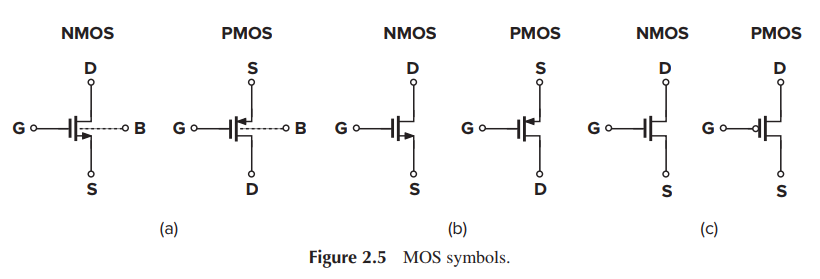
\includegraphics[width=\columnwidth]{NMOS_PMOS_Simbol}
        \label{图2}
        \caption{NMOS和PMOS图标}
    \end{figure}
    
\end{document}